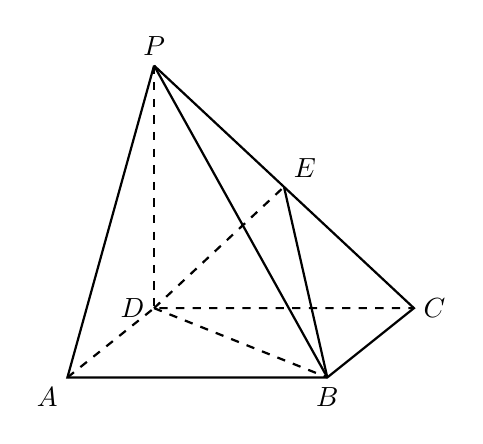
\begin{tikzpicture}[>=stealth, scale=1.1]
  % 顶点坐标
  \coordinate (D) at (1.0, 0.8);
  \coordinate (A) at (0, 0);
  \coordinate (B) at (3.0, 0);
  \coordinate (C) at (4.0, 0.8);
  \coordinate (P) at (1.0, 3.6);

  % 中点 E (PC 中点): P(1.0, 3.6), C(4.0, 0.8) -> E(2.5, 2.2)
  \coordinate (E) at (2.5, 2.2);

  % 实线棱
  \draw[thick] (P) -- (A) -- (B) -- (C) -- (P);
  \draw[thick] (P) -- (B);
  \draw[thick] (E) -- (B);

  % 虚线棱与辅助线
  \draw[dashed, thick] (P) -- (D);
  \draw[dashed, thick] (A) -- (D) -- (C);
  \draw[dashed, thick] (D) -- (B);
  \draw[dashed, thick] (D) -- (E);

  % 节点标注
  \node[above] at (P) {$P$};
  \node[below left] at (A) {$A$};
  \node[below] at (B) {$B$};
  \node[right] at (C) {$C$};
  \node[left] at (D) {$D$};
  \node[above right] at (E) {$E$};
\end{tikzpicture}
